\chapter{有限马尔科夫决策过程}\label{chap:3}

在本章中我们将介绍正式的有限卡尔科夫决策过程<finite Markov decision process, finite MDP>问题, 该问题正是我们在本书的余下部分中试图解决的. 这一问题即涉及到如赌博机问题中的评估性反馈, 又涉及到关联方面——在不同的情形下选择不同的动作. MDP\footnote{即使原文中MDP为复数, 即MDPs, 在译文中还是根据中文的语法, 不区分单复数, 仅写为MDP. 译者注.}是对系列决策过程的典型形式化, 其中动作不仅影响立即的奖赏, 也会影响此后的情形或者说是状态, 再以此影响未来的奖赏. 因此MDP涉及到延迟的奖赏, 需要就立即的奖赏与延迟的奖赏进行权衡. 在赌博机问题中, 我们评估每个动作$a$的值$q_*(a)$, 而在MDP中, 我们估计在各个状态$s$中各个动作$a$的值$q_*(s, a)$, 或者我们估计在最优动作选择下的各个状态的值$v_*(s)$. 这些依赖状态的量, 对于准确地将长期结果的赞誉<credit>分配给各个动作选择来说是必不可少的.

MDP是对强化学习问题进行的一种数学上的理想化, 可以在其中进行清晰的理论陈述. 我们将介绍强化学习问题的数学结构中的各个关键元素, 例如回报<return>, 值函数<value function>以及贝尔曼方程<Bellman equation>. 我们将尝试说明可以形式化为有限MDP的应用的范围之广. 正如整个人工智能领域, 此处也存在着应用的广度与数学上的易处理性这一对矛盾. 在本章中我们将会介绍这一对矛盾, 并讨论其中的一些权衡以及该矛盾所预示的挑战. 一些超出了MDP的强化学习方法将在\chapref{17}中被介绍.

% ----------------------------------- sec3.1 ---------------------------------------------
\section{代理-环境接口}\label{sec:3.1}

MDP意图成为``从与环境的交互中学习来达成目标''这一问题的直截了当的框架. 学习器以及决策者被称为\emph{代理}<agent>. 由代理之外的一切组成的、代理所交互的事物, 被称为\emph{环境}<environment>. 两者持续进行交互: 代理选择动作, 然后环境对动作做出反馈并将新的情形呈现给代理.\footnote{我们使用术语\emph{代理}、\emph{环境}以及\emph{动作}, 而非工程学中的术语\emph{控制器}<controller>, \emph{受控系统}<controlled system>(或\emph{设备}<plant>)以及\emph{控制信号}<control signal>, 因为前者所面向的受众更广.} 环境也给出了奖赏——代理希望通过动作选择来最大化积累量的、特殊的实数值. 

\begin{figure}[ht]
\centering
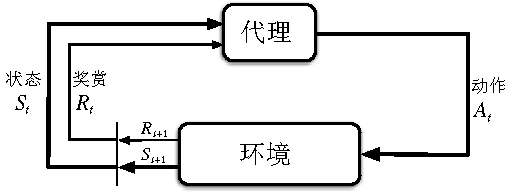
\includegraphics[width=.75\textwidth]{c3/img/figure3-1.pdf}
\caption{在马尔科夫决策过程中的, 环境与代理之间的交互.}\label{fig:3.1}
\end{figure}

% bib
更具体地说, 环境与代理在一系列离散的时步, $t = 0$, $1$, $2$, $3$, $\dots$\footnote{我们将注意力集中到离散时间序列这一情形上, 来使问题尽可能简单, 但许多概念可以拓展到连续时间的情形下(例如, 可以参见\cite{Bertsekas1996, Doya1996}).}, 上进行交互. 在每一时步$t$, 代理会接收到环境的\emph{状态}<state>$S_t \in \mathcal{S}$的某些表征, 并在此基础上选择一个\emph{动作}<action>$A_t \in \mathcal{A}(s)$\footnote{为了简化标记, 有时候我们假设在所有的状态上动作集是相同的, 并简单地将其写作$\mathcal{A}$.}. 在下一个时步, 某种程度上作为动作的结果, 代理会接收到一个实数型\emph{奖赏}<reward>$R_{t + 1} \in \mathcal{R} \subset \mathbb{R}$, 并发现自身处于一个新的状态$S_{t + 1}$中.\footnote{我们使用$R_{t + 1}$而非$R_t​$, 来表示这一奖赏归因于$A_t​$, 因为其强调了下一奖赏与下一状态$R_{t + 1}​$与$S_{t + 1}​$是联合被确定的. 不幸的是, 两者记法都在文献中被广泛使用.} 因此MDP与代理一起产生了如下的一系列轨迹:
\begin{equation}\label{eq:3.1}
S_0, A_0, R_1, S_1, A_1, R_2, S_2, A_2, R_3, \dots
\end{equation}
在\emph{有限}MDP中, 状态集、动作集与奖赏集($\mathcal{S}, \mathcal{A}, \mathcal{R}$), 都只有有限个元素. 在这一情形下, 随机变量$R_t$与$S_t$都有明确的离散概率分布, 且该分布仅依赖于前一状态与动作. 也就是说, 在给定前一状态与动作的情况下, 这两个随机变量的特定值$s' \in \mathcal{S}$及$r \in \mathcal{R}$, 出现的概率为:
\begin{equation}\label{eq:3.2}
p(s', r \mid s, a) \doteq \Pr (S_t = s', R_t = r \mid S_{t - 1} = s, A_{t - 1} = a),
\end{equation}
其适用于所有的$s', s \in \mathcal{S}, r \in \mathcal{R}, a \in \mathcal{A}(s)$. 函数$p$定义了MDP的\emph{动态}<dynamics>. 等式中等号上的点提醒我们这是一个定义式(在此情况下即为对函数$p$的), 而非由先前的定义推导出的事实. 动态函数$p : \mathcal{S} \times \mathcal{R} \times \mathcal{S} \times \mathcal{A} \rightarrow [0, 1]$, 是有4个参数的、一般的确定性函数. 其中的`$\mid$'为来自于条件概率的符号, 但在这里其仅用于提醒我们: $p$指明了各个$s$与$a$所带来的概率分布, 且
\begin{equation}\label{eq:3.3}
\sum_{s' \in \mathcal{S}} \sum_{r \in \mathcal{R}} p(s', r \mid s, a) = 1, \text{ 对所有的}s \in \mathcal{S}, a \in \mathcal{A}(s).
\end{equation}

在\emph{马尔科夫}决策过程中, 由$p$给出的概率可以完全确定环境的动态. 也就是说, $S_t$和$R_t$各个值的概率只由前一个状态与动作, 即$S_{t - 1}$和$A_{t - 1}$的具体值决定, 而不受更早的状态或动作任何影响. 最好不要将此视为决策过程上的约束, 而是视为\emph{状态}上的约束. 状态必须包括``过去代理与环境的交互中所有能对未来产生影响的方面''的信息. 如果符合此条件, 那么我们称这样的状态拥有\emph{马尔科夫性质}<Markov property>. 我们在整本书中都假设如此的马尔科夫性质, 虽然从\partref{2}开始我们将会学习不依赖于该性质的近似方法, 然后在\chapref{17}中我们将会阐述如何从非马尔科夫观测中, 学习并构建得马尔科夫状态.

从拥有4个参数的动态函数$p$中, 我们可以计算出任何和环境有关的想要的信息, 如\emph{状态转移概率}<state-transition probability>(虽然有滥用符号的嫌疑, 但我们使用有3个参数的函数$p: \mathcal{S} \times \mathcal{S} \times \mathcal{A} \rightarrow [0, 1]$来表示它),
\begin{equation}\label{eq:3.4}
p(s' \mid s, a) \doteq \operatorname{Pr}\{ S_t = s' \mid S_{t - 1} = s, A_{t - 1} = a \} = \sum_{r \in \mathcal{R}}p(s', r \mid s, a).
\end{equation}
我们可以计算出状态-动作对的期望奖赏, 并使用有2个参数的函数$r: \mathcal{S} \times \mathcal{A} \rightarrow \mathbb{R}$表示:
\begin{equation}\label{eq:3.5}
r(s, a) \doteq \mathbb{E}[R_t \mid S_{t - 1} = s, A_{t - 1} = a] = \sum_{r \in \mathcal{R}}r\sum_{s' \in \mathcal{S}}p(s', r \mid s, a),
\end{equation}
以及可以计算出针对状态--动作--下一状态三元组的期望奖赏, 并使用有3个参数的函数$r: \mathcal{S} \times \mathcal{A} \times \mathcal{S} \rightarrow \mathbb{R}$来表示:
\begin{equation}\label{eq:3.6}
r(s, a, s') \doteq \mathbb{E}[R_t \mid S_{t - 1} = s, A_{t - 1} = a, S_t = s'] = \sum_{r \in \mathcal{R}} r \frac{p(s', r \mid s, a)}{p(s' \mid s, a)} 
\end{equation}
在本书中, 我们常常使用\eqref{eq:3.2}中有4个参数的函数$p$, 但为了方便偶尔也使用其他的这些标记法.

MDP框架抽象而灵活, 可以以许多不同的方式应用到许多不同的问题中. 例如, 时步并不一定指代实际时间中的固定时间间隔; 其可以用于指代任意相继的关于决策与动作的场景. 动作可以是低层次的控制, 如加到机械臂的马达上的电压, 也可以是高层次的决策, 例如是否要吃午饭或是否去读研究生. 类似的, 状态也可以有各种各样的形式. 其可以完全由低层次的感知确定, 如传感器上的直接读数; 其也可以更加抽象且属于更加高层次, 例如对室内物体的符号性描述. 组成状态的事物可以基于对过去感知的记忆, 甚至可以完全是精神上的或主观的. 例如, 一个代理可以处于``不确定某物的位置''这么一个状态中, 或者可以从一个明确定义的角度``被吓了一跳''. 类似地, 一些动作也可以是精神上的或计算性的. 例如, 可能有一些动作可以控制代理思考的内容, 或控制代理的关注点. 一般来说, 动作可以是任何我们希望学得如何决策的决定, 而状态可以是任何我们认为可以帮助决策的事物. 

特别地, 代理与环境之间的界限, 通常不像机器人或动物体的物理界限那样. 通常来说, 该界限要近于物理界限. 例如, 机器人中的马达、机械联动装置以及传感硬件, 通常被认为是环境的一部分, 而非代理的一部分. 类似地, 如果我们将MDP框架用于人体或动物体, 肌肉、骨骼以及感知器官应该被认为是环境的一部分. 此外, 假设上说奖赏是在自然或人工学习系统的物理实体内部被计算, 但通常被认定为在代理的外部.

我们所遵循的一般规则为: 如果某物不能被代理任意改变, 那么该物被认为是在代理的外部, 因此也是环境的一部分. 我们并没有假设环境中的一切事物对于代理而言是未知的. 例如, 代理常常知道大量的关于``奖赏是怎样以一个动作与采取动作所在的状态的函数的形式被计算''的信息. 但我们总是认为奖赏的计算位于代理的外部, 因为其定义了代理所面对的任务, 因此代理没有对其进行任意修改的能力. 事实上, 在一些情况下, 代理可能知道环境运作的\emph{一切信息}, 但其面临的强化学习任务仍然非常困难, 例如我们完全知道魔方等谜题的规则, 但我们仍然无法解决它们. 代理与环境间的边界代表了代理的\emph{绝对控制能力}的限度, 而非其知识的限度.

代理与环境间的边界可以因不同的目的而置于不同的位置. 在一个复杂的机器人中, 可能有许多不同的代理同时进行操作, 而每一个都有其自身的边界. 例如, 一个代理做出了高层次的决策, 而这些高层次的决策组成了低层次的代理所面临的状态的一部分, 且正是由这些低层次的代理来实现高层次的决策. 实践中, 一旦特定的状态、动作与奖赏被选定, 代理与环境间的界限就确定下来了, 因此也确定了兴趣所在的特定决策任务.

MDP框架是对以目标为导向的、从交互中学习的问题的大幅度的抽象. 其指明——无论传感器、内存及控制装置的细节如何, 无论想要达到的目标是什么, 任何``学得目标导向的行为''这一问题可以简化为来回传递于代理与环境间的3个信号: 一个信号用于表示代理所做的决定(动作), 一个信号用于表示做出决定的基础(状态), 一个信号用于界定代理的目标(奖赏). 虽然这一框架不足以表示所有的决策问题, 但其已被证明能广泛地被应用.

当然, 不同任务中具体的状态与动作可能有巨大的差异, 且如何表示状态与动作可能会极大地影响性能. 在强化学习中, 就像在其他种类的学习中一样, 这样的关于表示的选择更像艺术而非科学. 在本书中, 我们会就``如何以好的方法来表示状态与动作''给出一些建议与例子, 但我们主要的关注点在于表示方式被选择后, 如何进行学习的一般准则.

\begin{exam}[例3.1 生物反应器]
假设强化学习用于决定生物反应器(用于产生有用的化学物质的一大堆营养物与细菌)中各个时刻的温度与搅拌速率. 在这样的一个应用中, 动作可以为控制目标温度与搅拌速率, 而控制是通过低层次的控制系统轮流激活加热元件或马达来实现的. 状态可以为(也许有延迟或经过了滤波的)热电偶以及其他传感器的读数, 连同代表桶中的原料与目标化学物质的符号性输入. 奖赏可以为生物反应器中各个时刻有用的化学物质产生的速率. 请注意其中每一个状态是传感器读数与符号性输入的列表或向量, 每一个动作是包含了目标温度与搅拌速率的向量. 对强化学习任务而言, 状态与动作拥有结构化的表示是很典型的. 而奖赏常常为单个数值.
\end{exam}

\begin{exam}[拾置机器人]
让我们考虑将强化学习用于控制反复的拾取-放置任务中机械臂的运动. 如果我们想要使机械臂学得快速而平滑的运动方式, 学习代理必须要能直接地控制马达, 且可以获得低延迟的关于机械联动装置当前的位置与速度的信息. 在这种情况下, 动作可能为加在机械臂的各个关节处的电压, 状态可能为各个关节的角度与速度的最新的读数. 如果一个物体被正确拾取并放置, 那么奖赏可以为+1. 为了激励平滑的动作, 可以在每一时步给出一个较小的负值奖赏, 并且该奖赏为运动的实时``颠簸度''的函数.
\end{exam}

\begin{exer}
写出3个适合于MDP框架的任务示例, 并给出各自的状态、动作与奖赏. 尽可能使3个示例有较大的差异. MDP框架抽象而灵活, 可以以多种方式使用. 在至少一个实例中以某种方式逼近MDP框架的极限.
\end{exer}

\begin{exer}
MDP框架足以表示\emph{所有}的目标导向的学习任务吗? 你可以想出任何明确的反例吗?
\end{exer}

\begin{exer}
现在考虑关于驾驶的问题. 你可以从油门、刹车和方向盘的角度, 即从身体与汽车的接触的角度, 来定义动作. 或者你可以从更为外侧的角度来定义动作——例如从轮胎的橡胶与路面的接触的角度看, 将动作设定为控制轮胎的扭矩. 或者你也可以从更为内侧的角度来定义动作——例如从大脑与身体的交互的角度看, 将动作定义为收缩肌肉以控制四肢. 或者你可以从相当高层次的角度看, 将动作定义为对驶向\emph{何处}的选择. 应该在哪一个层次或哪里对划定代理与环境的界限? 有没有偏好某一划分的根本理由, 或者说是可以随意选择?
\end{exer}

\hypertarget{exam:3.3}{}
\stepcounter{examcnt}%
\begin{mathbox}{例\theexamcnt: 回收机器人}
有一个在办公室中收集汽水罐的移动机器人. 该机器人有用于发现汽水罐的传感器, 以及用于拾取汽水罐并将汽水罐置于携带的垃圾箱中的机械臂与夹子; 其使用可充电电池. 该机器人的控制系统有用于理解传感信息、用于导航以及用于控制机械臂与夹子的组件. 基于电池的当前电量, 强化学习代理做出如何搜索汽水罐这样的高层次决定. 举一个简单的例子, 假设仅有两种电量等级可以被区分, 这两者组成了一个简单的状态集$\mathcal{S} = \{ \mathtt{high, low} \}$. 在每一个状态中, 代理可以决定是(1)积极地在一段时间内\texttt{搜索}<\texttt{search}>汽水罐, 或是(2)保持静止并\texttt{等待}<\texttt{wait}>别人过来扔汽水罐, 还是(3)返回据点并对电池进行\texttt{充电}<\texttt{recharge}>. 当电量等级为\texttt{high}时, 进行充电是一件愚蠢的事, 所以我们不将其包括在该状态的动作集中. 因此动作集为$\mathcal{A}(\mathtt{high}) = \{ \mathtt{search, wait} \}$以及$\mathcal{A}(\mathtt{low}) = \{ \mathtt{search, wait, recharge} \}$.

在多数时间内奖赏为0, 但是当机器人获得了一个空罐时其为正值, 当电量耗尽则其为一个绝对值较大的负值. 发现汽水罐的最好的方法就是积极地进行搜索, 但这会消耗机器人的电量, 而等待则不会消耗电量. 当机器人在搜索时, 有电量耗尽的可能. 如果电量耗尽, 那么机器人必须停机并等待援助(产生一个负奖赏). 如果电量等级为\texttt{high}, 那么机器人总是可以进行一段时间的积极搜索而没有电量耗尽的风险. 如果起始电量等级为\texttt{high}, 在经过一段时间的搜索后, 电量等级以$\alpha$的概率维持在\texttt{high}, 而以$1 - \alpha$的概率减为\texttt{low}. 在另一方面, 如果起始电量等级为\texttt{low}, 那么在经过一段时间的搜索后, 电量等级以$\beta$的概率维持在\texttt{low}, 而以$1 - \beta$的概率耗尽. 在后一种情况下, 机器人必须等待援助, 且电量在充电后恢复为\texttt{high}. 机器人收集的每个汽水罐都会产生单位奖赏, 而当机器人必须被援助时, 会产生$-3$的奖赏. 让我们使用$r_{\mathtt{search}}$和$r_{\mathtt{wait}}$(其中$r_{\mathtt{search}} > r_{\mathtt{wait}}$)来分别表示搜索与等待可以获得的汽水罐的期望数量(因此也是奖赏的期望值). 最后, 假设在机器人回据点的路上或机器人电量耗尽时, 其不能收集任何汽水罐. 那么这一系统就成为了有限MDP, 我们可以获得转移概率与期望的奖赏, 其中动态如下表所示:

\begin{center}
\begin{minipage}[c]{.5\textwidth}
\includegraphics[width=\textwidth]{c3/img/dynamics_table.pdf}
\end{minipage}
\quad
\begin{minipage}[c]{.45\textwidth}
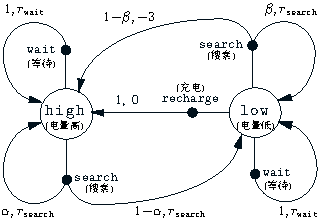
\includegraphics[width=\textwidth]{c3/img/mdp.pdf}
\end{minipage}
\end{center}
\vspace{.5em}

当前状态$s$, 动作$a \in \mathcal{A}(s)$, 及下一个状态$s'$的每一种可能的组合都对应于表中的一行. 另一种概括有限MDP动态的有用工具为如上所示的\emph{转移图}<transition graph>. 其中有两种结点: \emph{状态结点}与\emph{动作结点}. 每一个可能的状态都对应于一个状态结点(使用状态名标记的大的白圈), 每一个状态-动作对都对应于一个动作结点(连接到状态结点的、由动作名标记的小的实心圈). 于状态$s$采取动作$a$, 对应于转移图就是从状态结点$s$开始沿线移动到动作结点$(s, a)$. 然后环境通过离开动作结点$(s, a)$的箭头之一来做出响应并转移到下一个状态状态. 每一个箭头都对应于一个三元组$(s, s', a)$, 其中$s'$是下一个状态, 然后我们使用转移概率$p(s' \mid s, a)$以及该转移的期望奖赏$r(s, a, s')$来对箭头进行标记. 请注意所有离开同一个动作结点的箭头上标注的转移概率的和一定为1.
\end{mathbox}

\begin{exer}
类比于\hyperlink{exam:3.3}{例3.3}中的表, 绘制针对$p(s', r \mid s, a)​$的表格. 该表应该有$s​$, $a​$, $s'​$, $r​$以及$p(s', r \mid s, a)​$这些列, 并且每一个$p(s', r \mid s, a) > 0​$的四元组都应该有对应的行.
\end{exer}

% ----------------------------------- sec3.2 ---------------------------------------------
\section{目标与奖赏}\label{sec:3.2}

在强行学习中, 代理的目的或目标是使用一个特殊的被称为\emph{奖赏}<reward>的信号来形式化的, 且该信号由环境传给代理. 在每一时步, 奖赏就是简单的一个数值, $R_t \in \mathbb{R}$. 不那么正式地说, 代理的目标就是最大化接受到的奖赏总量. 这意味着不是最大化立即奖赏, 而是最大化长期的累积奖赏. 我们可以将这一非正式的理念阐述为\emph{奖赏假定}<reward hypothesis>:
\begin{quote}
我们所说的目标或目的可以完全被理解为: 最大化收到的标量信号(称为奖赏)的累积量的期望值.
\end{quote}
使用奖赏信号来形式化目标的概念, 是强化学习最显著的特征之一.

虽然使用奖赏信号来形式化目标可能初看上去颇具有局限性, 但在实践中其已被证明灵活且广泛可用. 来展示这一点的最好方法就是考虑一些此方法曾被如何使用或能被如何使用的例子. 例如, 为了使机器人学会走路, 研究者设定在每一时步给予正比于机器人前向移动距离的奖赏. 为了使机器人学得如何从迷宫中逃脱, 在逃离前的每个时步中奖赏都是$-1$: 这激励机器人尽快逃脱. 为了使机器人学得如何发现并收集空汽水罐以回收利用, 我们可以在多数的时间下给予其0的奖赏, 而其每收集一个汽水罐, 就给予其$+1$的奖赏. 我们也可以在机器人撞到东西或被人责骂时给予其负值的奖赏. 为了使代理学会玩西洋跳棋或国际象棋, 一个自然的选择就是获胜时给予$+1$的奖赏, 失败时给予$-1$的奖赏, 而在平局时或下棋过程中给予0的奖赏.

你可以看到在这些例子中所发生的事情. 代理总是以最大化奖赏为目标进行学习. 如果我们希望代理为我们做些什么, 我们必须以这样的原则为其提供奖赏——通过最大化累积奖赏代理能达成我们的目标. 因此, 我们设定的奖赏能否真实反映我们我们希望达成的目标就显得至关重要了. 特别来说, 奖赏信号不是将\emph{怎样}达成目标的先验知识传递给代理的地方.\footnote{更好的引入此类先验知识的地方在初始策略之处, 初始值函数之处, 或能影响这两者的地方.} 例如, 下棋代理只有在真正获胜的时候才能获得奖赏, 而不能在达成例如``吃掉了对手的棋子''或``占据了棋盘的中间位置''之类的子目标时获得奖赏. 如果在达成这类子目标时获得了奖赏, 那么代理有可能寻得达成了子目标、却没有达成真正的目标的方式. 例如, 代理可能吃了对手的棋子, 但代价是失去了比赛. 通过奖赏信号的方式, 你告诉代理你希望其达成\emph{什么}目标, 而不是你希望其\emph{如何}达成目标.

% ----------------------------------- sec3.3 ---------------------------------------------
\section{累积奖赏与分节}\label{sec:3.3}

迄今为止, 我们已经非正式地讨论了学习的目标. 我们说过代理的目标就是从长期而言, 最大化其接收的累积奖赏. 那么这怎样被正式定义呢? 如果时步$t$后接收的奖赏序列记为$R_{t + 1}$, $R_{t + 2}$, $R_{t + 3}$, $\dots$, 那么我们希望最大化这一序列的具体的哪一方面? 一般而言, 我们希望最大化\emph{期望回报}, 其中回报<return>\footnote{在余下的译文中``回报''一般为强化学习专有术语, 专指此处的return. 译者注}记为$G_t$, 被定义为奖赏序列的某一具体函数. 在最简单的情况下回报就是奖赏的和:
\begin{equation}\label{eq:3.7}
G_t \doteq R_{t + 1} + R_{t + 2} + R_{t + 3} + \dots + R_T,
\end{equation}
其中$T$为最后一个时步. 这种方式对``能自然地定义最终时步''这样的应用而言才有意义, 也就是说, 当代理与环境的交互可以自然地划分为不同的子序列时才有意义, 我们将这样的子序列称为\emph{分节}<episode>,\footnote{在文献中, 分节有时也被称为``试验''<trial>.} 例如一局比赛, 一次穿越迷宫的历程, 或任意类型的重复的交互. 每一个分节都以被称为\emph{末状态}<terminal state>的特殊状态终止, 然后重置为标准的起始状态, 或重置为对起始状态的标准分布的某一采样. 虽然分节可能以多种方式结束, 例如赢得比赛或失去比赛, 但无论上一分节是如何结束的, 紧接着的分节如何起始与此毫无关系. 因此所有的分节可以认为是在相同的末状态结束的, 只是对不同的结果而言有不同的奖赏. 具有不同分节的任务被称为分节式任务<episodic task>. 在分节式任务中, 我们有时需要将记为$\mathcal{S}$的非末状态的集合, 与记为$\mathcal{S}^+$的包括末状态的所有状态的集合区分开来. 终止的时间$T$, 通常是随分节不同而不同的随机变量

另一方面, 在许多情形下, 代理与环境的交互不能自然地划分为可辨别的分节, 而是没有限制地永远进行下去. 例如, 可以很自然地以此种方式形式化一个持续进行的过程控制任务, 或一个长生命周期的机器人应用. 我们将这样的任务称为\emph{持续式任务}<continuing task>. 对持续式任务来说, 回报公式\eqref{eq:3.7}是有问题的, 因为最终时步$T = \infty$, 且我们希望最大化的回报可以很轻易地为无穷大. (例如, 假设代理在每一时步都接收到+1的奖赏.) 因此, 本书中我们经常使用的那种回报的定义, 在概念上稍微更为复杂, 但数学上简单了很多. 

我们需要额外概念为\emph{折扣}<discount>. 据此, 代理以最大化未来接收到的折扣后奖赏的和为目标, 来进行动作选择. 特别地, 代理选择$A_t$以最大化期望的\emph{折扣后回报}:
\begin{equation}\label{eq:3.8}
G_t \doteq R_{t + 1} + \gamma R_{t + 2} + \gamma^2 R_{t + 3} + \dots = \sum_{k = 0}^{\infty} \gamma^k R_{t + k + 1},
\end{equation}
其中$0 \leq \gamma \leq 1$, $\gamma$被称为\emph{折扣率}<discount rate>.

折扣率决定了未来奖赏的当前值: 在$k$个时步后接收到的奖赏, 为立即接收到的同样的奖赏的$\gamma^{k - 1}$倍. 如果$\gamma < 1$, 那么只要奖赏序列$\{ R_k \}$是有界的, \eqref{eq:3.8}中的无限项的和就是一有限值. 如果$\gamma = 0$, 那么代理因仅关心于最大化立即奖赏而变得``短视'': 在这种情况下, 代理的目标即为选择$A_t$以仅仅最大化$R_{t + 1}$. 如果代理的每一个动作恰巧仅影响立即奖赏而不会影响未来奖赏, 那么一个短视的代理可以通过分别最大化每一个立即奖赏来最大化\eqref{eq:3.8}. 但是一般来说, 为了最大化立即奖赏而选择动作, 会减少将来的奖赏, 因而减少回报. 当$\gamma$趋近于1时, 回报的目标更多地将未来的奖赏考虑在内, 即代理的目光变得更为长远.

相邻时步中的回报彼此相关, 其相关的方式对强化学习的理论与算法来说十分重要:
\begin{equation}\label{eq:3.9}
\begin{aligned}[b]
G_t &\doteq R_{t + 1} + \gamma R_{t + 2} + \gamma^2 R_{t + 3} + \gamma^3 R_{t + 4} \dots \\
&= R_{t + 1} + \gamma (R_{t + 2} + \gamma R_{t + 3} + \gamma^2 R_{t + 4} + \dots) \\
&= R_{t + 1} + \gamma G_{t + 1}
\end{aligned}
\end{equation}
请注意如果我们定义$G_T = 0$, 那么这对所有的$t < T$的时步都成立, 即使终止发生于$t + 1$. 这使得由奖赏序列计算回报变得容易.

请注意虽然\eqref{eq:3.8}中的回报由无穷多项组成, 但如果奖赏为非0常数, 且$\gamma < 1$, 那么回报值仍是有限的值. 例如, 如果奖赏恒定为+1, 那么回报为
\begin{equation}\label{eq:3.10}
G_t = \sum_{k = 0}^{\infty} \gamma^k = \frac{1}{1 - \gamma}
\end{equation}

\begin{exer}
\secref{3.1}中的等式是针对于持续式任务的, 如果想要将其用于分节式任务中的话, 需要对其进行(非常小的)修改. 通过给出\eqref{eq:3.3}修改后的版本来证明你知道如何进行修改. 
\end{exer}

\begin{wrapfigure}[6]{r}{.45\textwidth}
\centering
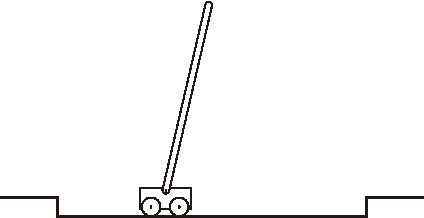
\includegraphics[width=.4\textwidth]{c3/img/pole-balancing.pdf}
\end{wrapfigure}
\mbox{}~
\begin{exam}[杆之平衡]
本任务的目标为在一个沿轨道移动的小车上施加合适的力, 使得铰接于小车上的杆子不会落倒: 如果杆子与垂直方向的夹角超过了给定值, 或小车跑出了轨道, 那么就算作失败. 每次失败后杆子都会重置到垂直方向上. 可以以分节式的方式处理该任务, 其中重复进行的将杆保持平衡的尝试, 就是自然划分的分节. 在这种情况下, 尚未失败的时步中奖赏为$+1$, 那么每一时步中的回报就是距离失败所余下的步数. 这样的话, 如果杆能永远保持平衡, 那么回报就会趋于无穷大. 作为代替, 我们可以使用折扣, 将此任务作为持续式任务对待. 在这种情况下, 每次失败时奖赏为$-1$, 而所有的其他时步中奖赏为0. 那么在每一时步中, 回报将和$- \gamma^K$相关, 其中$K$为距离失败的时步数. 无论在哪种情况下, 都是令杆尽可能长时间地保持平衡来最大化回报.
\end{exam}

\begin{exer}
假设你将杆之平衡作为分节式任务对待, 但同时也使用折扣, 且除了失败时奖赏为$-1$外, 其他所有时间奖赏为0. 那么每一时步中的回报将会是如何? 该回报将与本任务上折扣、连续式的设定下的回报有何区别?
\end{exer}

\begin{exer}
假设你在设计一个走迷宫的机器人. 你决定在其逃出迷宫时给予$+1$的奖赏, 而在所有的其他时间均给予0的奖赏. 这个任务看上去可以很自然地划分为各个分节——即相继的走迷宫的尝试——所以你决定将其作为分节式任务对待, 其中目标就是最大化期望的奖赏和\eqref{eq:3.7}. 在令代理尝试走一段时间的迷宫后, 你发现其在逃离迷宫方面没有任何改进. 哪里出错了呢? 你有没有真正地将你的目标传达给代理?
\end{exer}

\begin{exer}
假设$\gamma = 0.5$, 且接收到了如下的奖赏序列: $R_1 = -1$, $R_2 = 2$, $R_3 = 6$, $R_4 = 3$以及$R_5 = 2$, 其中$T = 5$. 那么$G_0, G_1, \dots, G_5$为多少? 提示: 从后往前算.
\end{exer}

\begin{exer}
假设$\gamma = 0.9$, 且接收到的奖赏序列为: $R_1 = 2$, 之后为无数多个7. 那么$G_1$和$G_0$的值为多少?
\end{exer}

\begin{exer}
证明\eqref{eq:3.10}中的第二个等号.
\end{exer}

% ----------------------------------- sec3.4 ---------------------------------------------
\section{分节式与持续式任务的统一标记方式}\label{sec:3.4}

在前一节我们介绍了两种强化学习任务: 一种中代理与环境间的交互可以自然地划分为独立的分节(分节式任务), 而另一种中并非如此(持续式任务). 前一种情况从数学上说更为简单, 因为每个动作仅影响该分节中随后接收到的有限个奖赏. 在本书中, 我们有时考虑一种, 有时考虑另一种, 但常常是两种一起考虑. 因此建立一种能同时精确地用于两种情形的标记方式就显得很有帮助了.

我们需要一些额外的标记来更清楚地表示分节式任务. 对于分节式任务, 我们不能将其考虑为由时步组成的单个长序列, 而是考虑为一系列的分节, 其中每一个分节都由有限的时步序列组成. 在每一个分节开始时, 我们重新从0开始对时步进行计数. 因此, 仅使用$S_t$, 即时步$t$处的状态, 来进行指代是不够的, 我们需要使用$S_{t, i}$, 即分节$i$中的时步$t$处的状态, 来进行指代(类似地, 有$A_{t, i}$, $R_{t, i}$, $\pi_{t, i}$, 以及$T_i$等等). 然而, 事实上当我们讨论分节式任务时我们几乎不用对各个分节进行区分. 我们几乎总是仅考虑单个特定分节, 或者我们所论述的对所有的分节都成立. 因此, 实践中我们总是轻微地滥用标记: 省去了分节的具体索引. 也就是说, 我们使用$S_t$时, 我们指的是$S_{t, i}$, 其余的也类似.

为了得到分节式与持续式任务的统一标记方式, 我们还需要另一个规约. 在情形\eqref{eq:3.7}下, 我们将回报定义为有限个项的和; 而在情形\eqref{eq:3.8}下, 我们将其定义为无限个项的和. 如果我们将分节的终结视为进入了一个特殊的\emph{吞没状态}<absorbing state>, 即仅转移到自身且获得的所有奖赏均为0的状态, 那么我们可以将两种任务统一起来. 例如, 考虑如下的转移图:

\begin{figure}[ht]
\centering
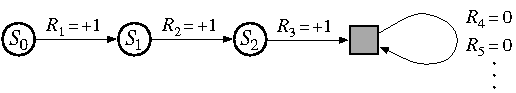
\includegraphics[width=.7\textwidth]{c3/img/transition_graph.pdf}
\end{figure}

其中实心的方框表示对应于分节的终止的、特别的吞没状态. 从$S_0$开始, 我们获得了奖赏序列$+1$, $+1$, $+1$, $0$, $0$, $0$, $\dots$. 那么仅对前$T$个奖赏求和的值(此处$T = 3$), 同对整个无穷项的序列求和的值是一样的. 即使我们引入折扣, 这同样成立. 因此, 我们可以以如下方式定义一般性的回报: 依据于式\eqref{eq:3.8}; 并且依照``当不需要分节的编号时将其省略"这一惯例; 同时如果和有定义, 那么保留$\gamma = 1$的可能(例如, 如果所有的分节都会终止, 那么可以这么做). 作为代替, 我们可以获得
\begin{equation}\label{eq:3.11}
G_t \doteq \sum_{k = t + 1}^{T} \gamma^{k - t - 1} R_k,
\end{equation}
其中$T= \infty$或$\gamma = 1$都是被允许的(但不能两者同时). 我们在的本书的余下内容中使用这一惯例, 以简化标记并展示分节式任务与持续式任务的高度并行性. (更晚些, 在\chapref{10}中, 我们将介绍连续且非折扣的表述方式.)

% ----------------------------------- sec3.5 ---------------------------------------------
\section{策略与值函数}\label{sec:3.5}

几乎所有的强化学习算法都涉及到对值函数——估计对代理而言给定状态的\emph{好坏程度}的, 以状态为参数的函数(或估计在给定状态执行给定动作的好坏程度的, 以状态-动作对为参数的函数)——进行估计. 这里``好坏程度"的概念是就可以期待的未来奖赏定义的, 或更准确地说, 就期望回报定义的. 当然, 代理所期望的能在未来接收到的奖赏, 依赖于其所采取的动作. 因此, 值函数被定义为同具体的采取动作的方式——即策略——相关.

正式地说, \emph{策略}<policy>是从状态到选择各个可能动作的概率的映射. 如果代理在时步$t$使用策略$\pi$, 那么$\pi(a \mid s)$即为当$S_t = s$时$A_t = a$的概率. 就像$p$一样, $\pi$也是一个普通的函数; $\pi(a \mid s)$中的``$\mid$"仅用于提醒我们: 该函数为每一个$s \in \mathcal{S}$定义了$a \in \mathcal{A}(s)$上的概率分布. 由强化学习方法指定代理的策略如何根据经历来调整.

\begin{exer}
如果当前状态为$S_t$, 并且根据概率性策略$\pi$来进行动作选择, 那么如何用$\pi$以及4参数的函数$p$\eqref{eq:3.2}来表示$R_{t + 1}$的期望值?
\end{exer}

在策略$\pi$下状态$s$的值函数, 记为$v_\pi(s)$, 为从状态$s$开始, 并在之后遵循策略$\pi$, 而获得的期望回报. 对于MDP, 我们可以用下式正式定义$v_\pi$:
\begin{equation}\label{eq:3.12}
v_\pi(s) \doteq \mathbb{E}_\pi[G_t \mid S_t = s] = \mathbb{E}_\pi \left[ \sum_{k = 0}^{\infty} \gamma^k R_{t + k + 1} \mid S_t = s \right], \text{对所有的}s \in \mathcal{S},
\end{equation}
其中$\mathbb{E}_\pi [\cdot]$表示当代理使用策略$\pi$时随机变量的期望值, 而$t$为任一时步. 如果有吞没状态的话, 那么该状态的值一定为0. 我们将函数$v_\pi$称为\emph{针对策略$\pi$的状态值函数}<state-value function>. 

类似的, 我们将策略$\pi$下在状态$s$中采取动作$a$的值, 定义为从状态$s$开始, 采取动作$a$, 并在之后遵循策略$\pi$, 而可以获得的期望回报, 并将其记为$q_\pi(s, a)$:
\begin{equation}\label{eq:3.13}
q_\pi(s, a) \doteq \mathbb{E}_\pi[G_t \mid S_t = s, A_t = a] = \mathbb{E}_\pi \left[ \sum_{k = 0}^{\infty} \gamma^k R_{t + k + 1} \mid S_t = s, A_t = a \right].
\end{equation}
我们将$q_\pi$称为\emph{针对策略$\pi$的动作值函数}<action-value function>.

\begin{exer}
使用$q_\pi$和$\pi$来表示$v_\pi$.
\end{exer}

\begin{exer}
使用$v_\pi$和4参数函数$p$来表示$q_\pi$.
\end{exer}

值函数$v_\pi$与$q_\pi$可以利用经历来进行估计. 例如, 如果对遇到的每一个状态, 记录该状态随后的实际回报, 然后计算均值, 那么当遇到该状态的次数趋于无穷大时, 均值也会收敛到该状态的值$v_\pi(s)$. 如果对每一个状态中的各个动作分别计算均值, 那么这些均值也会类似地收敛到$q_\pi(s, a)$. 我们将此类估计方式称为\emph{蒙特卡洛方法}<Monte Carlo method>, 因为此类方法涉及到对大量实际回报值的随机样本进行平均. 此类方法将会在\chapref{5}中进行介绍. 当然, 如果有许多状态的话, 那么为每个状态各自维持一个均值是不切实际的. 作为代替, 代理将以参数化函数的形式(参数个数必须少于状态个数)来维持$v_\pi$与$q_\pi$, 并调整参数来更好地与观测到的回报匹配. 这样也可以产生精确的估计值, 但这极其依赖于参数化函数近似器的种类. 这些内容将在本书的\partref{2}讨论.

一条贯穿于强化学习与动态规划始终的, 关于值函数的基本性质为: 其满足类似于我们已经讨论过的回报公式\eqref{eq:3.9}那样的递归关系. 对任意策略$\pi$和任意状态$s$来说, 下述的一致性条件在$s$的值与其可能的后一状态的值间成立:
\begin{align}
v_{\pi}(s) &\doteq \mathbb{E}_{\pi}[G_t \mid S_t = s] \nonumber\\
&= \mathbb{E}_{\pi}[R_{t + 1} + \gamma G_{t + 1} \mid S_t = s]  \tag*{\text{通过$\eqref{eq:3.9}$}}\nonumber\\
&= \sum_a \pi(a \mid s) \sum_{s'}\sum_{r}p(s', r \mid s, a) \Big[r + \gamma \mathbb{E}_{\pi}[G_{t + 1} \mid S_{t + 1} = s'] \Big]  \nonumber\\
&= \sum_a \pi(a \mid s) \sum_{s', r}p(s', r \mid s, a)\Big[ r + \gamma v_{\pi}(s') \Big], \text{ 对所有的} s \in \mathcal{S}, \label{eq:3.14}
\end{align}
且其中隐含着以下几点: 动作$a$来自于集合$\mathcal{A}(s)$, 下一状态$s'$来自于集合$\mathcal{S}$(在分节式问题中来自集合$\mathcal{S}^+$), 奖赏$r$来自于集合$\mathcal{R}$. 请注意在最后一个等式中, 我们是怎么将两个和式——一者为在$s'$的所有值上求和, 另一者为在$r$的所有值上求和——归并到对两者的所有可能值求和. 我们常常使用这种归并后的和式来简化公式. 也请注意对最后那个表达式, 我们可以轻易地将其作为期望值来理解. 实际上其为在三个变量$a$, $s'$与$r$的所有值上的和式. 对每一个三元组, 我们计算其概率$\pi(a \mid s)p(s', r \mid s, a)$, 并将该概率作为方括号内值的权重, 然后在所有的概率上求和来得到期望值. 

\begin{wrapfigure}{r}{.3\textwidth}
\centering
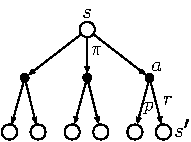
\includegraphics[width=.3\textwidth]{c3/img/backup_diagram.pdf}\\
对$v_{\pi}$的逆流图
\end{wrapfigure}
等式\eqref{eq:3.14}为\emph{针对$v_{\pi}$的贝尔曼方程}<Bellman equation>. 其阐述了某一状态的值与其各个后一状态的值间的关系. 试想下从某一个状态向前看, 看到了所有可能的后一状态的情形, 如右图所示. 每一个空心圆代表了一个状态, 而每一个实心圆代表了一个动作-状态对<state-action pair>. 从最上方的作为根结点的状态$s$出发, 代理可以基于其策略$\pi$选择某一动作集中的任何一个动作——图中展示了3个这样的动作. 从任一动作出发, 环境会反馈以数个下一状态(在图中展示了两个)中的选择, 即$s'$, 以及依据由函数$p$给出的动态得到的奖赏$r$. 贝尔曼方程\eqref{eq:3.14}以概率为权重, 在所有可能性上求和. 其显示出: 一状态的值一定等于其下一状态的(未经折扣的)值与随同的奖赏这两者之和的期望值.

值函数$v_{\pi}$是其贝尔曼方程的唯一解. 我们将在后续的章节中展示: 贝尔曼方程何以成为数种计算、近似与学习$v_{\pi}$的方法的基础. 我们将上面出现过的那种图称为\emph{逆流图}<backup diagram>, 因为其绘制出的关系构成了更新或\emph{逆流}<backup>操作的基础, 而该操作为强化学习方法的核心. 这些操作将值的信息从某一状态的后一状态(或动作-状态对), 逆向传输到该状态(或状态-动作对). 我们将在本书中持续使用逆流图, 来提供对正在讨论的算法的图形化概述. (请注意, 不像转移图, 逆流图中的状态结点并不一定表示不同的状态; 例如, 一个状态的后一状态可能为其本身.)

\hypertarget{exam:3.5}{}
\begin{exam}[网格世界]
\figref{3.2}(左)展示了一矩形的网格世界以作为有限MDP的简单示例. 网格中的每一个小格都对应于环境中的状态. 在一个小格上, 有4种可能的动作: \textbf{北移}, \textbf{南移}, \textbf{东移}, 以及\textbf{西移}, 其中各个动作都确定性地使代理在网格上沿对应的方向移动一格. 如果所采取的动作将令代理脱离网格, 那么该动作的结果为代理的位置保持不变, 且造成$-1$的奖赏. 除了上述动作与将代理移出特殊状态\textsf{A}与\textsf{B}的动作外, 其他的动作只会造成0的奖赏. 在状态\textsf{A}上, 所有的4个动作会产生$+10$的奖赏, 并将代理带至\textsf{A'}. 在状态\textsf{B}上, 所有的4个动作会产生$+5$的奖赏, 并将代理带至\textsf{B'}.

\begin{figure}[htb]
\centering
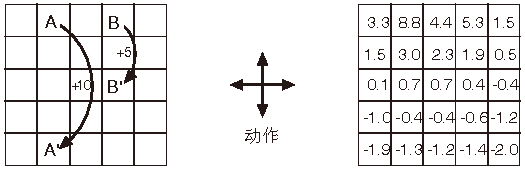
\includegraphics[width=.8\textwidth]{c3/img/figure3-2.pdf}
\caption{网格世界的例子: 例外的奖赏动态(左)与等可能性随机策略的状态值函数(右)}\label{fig:3.2}
\end{figure}

假设在所有的状态中, 代理都以相等的概率选择所有的4个动作. \figref{3.2}展示了在$\gamma = 0.9$的折扣情形下, 针对这一策略的值函数$v_{\pi}$. 此函数是通过解线性方程组\eqref{eq:3.14}得到的. 请注意在下方边界上的负值: 这是在本随机策略下代理有较大的可能撞到网格的边界所导致的结果. 状态\textsf{A}为本策略下最好的状态, 但其值小于10, 即小于其立即奖赏, 这是因为从状态\textsf{A}代理会被带至\textsf{A'}, 而在\textsf{A'}代理很可能会撞到网格的边界. 另一方面, 状态\textsf{B}的值大于5, 即大于其立即奖赏, 这是因为从状态\textsf{B}代理会被带至\textsf{B'}, 而状态\textsf{B'}的值为正. 从B开始因撞到边界而产生的期望惩罚值(负的奖赏)不及误打误撞进入\textsf{A}或\textsf{B}而产生的期望奖赏.
\end{exam}

\begin{exer}
就\examref{3.5}中\figref{3.2}(右)所示的值函数$v_{\pi}$而言, 贝尔曼方程\eqref{eq:3.14}一定对每一个状态都成立. 从数值上来证明, 就值分别为$+2.3$, $+0.4$, $-0.4$, $+0.7$的相邻状态而言, 贝尔曼方程在值为$+0.7$的正中间的状态上成立. (这些数值都只保留了1位有效数字.)
\end{exer}

\begin{exer}
在网格世界的例子中, 当离开目标状态时奖赏为正, 当撞到世界的边界时奖赏为负, 且在余下的时间内奖赏为0. 是这些奖赏的正负重要, 还是只有奖赏间的差值重要? 使用\eqref{eq:3.8}来证明向所有的奖赏加上一个常数$c$, 将会令所有状态的值增加一常数$v_c$, 因此不影响任意策略下的任意状态间的差值. 如何用$c$和$\gamma$来表示$v_c$?
\end{exer}

\begin{exer}
现在考虑在一个如走迷宫的分节式任务中, 向所有的奖赏加上一个常数$c$. 这会有什么影响, 还是像持续式任务中那样使得任务保持不变? 为什么或为什么不? 请给出一个例子.
\end{exer}


\begin{exam}[高尔夫]
\begin{figure}[htb]
\centering
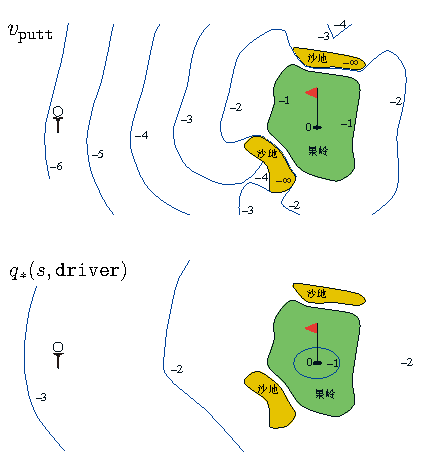
\includegraphics[width=.6\textwidth]{c3/img/figure3-3.pdf}
\caption{一个高尔夫的例子: 仅推球的状态值函数(上方)与使用木杆的最优动作值函数(下方)).}\label{fig:3.3}
\end{figure}
为了将打高尔夫球形式化为强化学习任务, 我们令每一杆都有$-1$的惩罚值(负的奖赏), 直到球进洞为止. 状态为球的位置. 状态的值为从当前位置到进洞所需的杆数的相反数. 我们的动作为如何进行瞄准与击球, 以及我们选择什么样的球杆. 让我们假定前者是给定的, 只需考虑球杆的选择, 其中我们假设要么选择推杆<\texttt{putter}>, 要么选择木杆<\texttt{driver}>. \figref{3.3}中的上半部分展示了总使用推杆时的状态值函数$v_{\mathtt{putt}}$. \emph{位于洞中}这一吞没状态值为0. 假设可以从果岭\footnote{果岭是高尔夫球运动中的一个术语, 是指球洞所在的草坪, 果岭的草短、平滑, 有助于推球. 果岭\\为英文green音译而来, 对应于\figref{3.3}中的绿色部分. 译者注.}的任意一处推球入洞; 这些状态的值为$-1$. 在果岭之外, 我们不能仅一杆就推球入洞, 因此状态值的绝对值更大. 如果我们可以靠一次推球进入果岭, 那么该状态的值一定比果岭的状态值小1, 即值为$-2$. 为了简洁起见, 让我们假设我们可以十分精确与确定性地推球, 但距离有限. 这为我们给出了图中标着$-2$的尖锐轮廓线; 所有介于该轮廓线与果岭之间的位置都需要恰好2杆来使球进洞. 类似地, 任一可以通过一次推球到达$-2$轮廓线的位置的值一定为$-3$, 并以此类推来得到图中所示的所有轮廓线. 推球并不能将球推出沙坑, 因此该状态值为$-\infty$. 总体而言, 从球座到洞我们共需要6杆. 
\end{exam}

\begin{wrapfigure}[3]{r}{.16\textwidth}
\centering
\vspace{-0.7em}
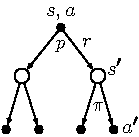
\includegraphics[width=.16\textwidth]{c3/img/action_value_backup_diagram.pdf}\\
{\tiny 针对$q_{\pi}$的逆流图}
\end{wrapfigure}
\mbox{}~
\begin{exer}
针对动作值$q_{\pi}$的贝尔曼方程是怎样的? 其中动作值$q_{\pi}(s, a)$必须用$(s, a)$的所有可能的后一动作-状态对的动作值$q_{\pi}(s', a')$来表示. 提示: 右侧的逆流图对应于这一方程. 请给出类似于\eqref{eq:3.14}的针对动作值的等式推导过程.
\end{exer}

\begin{exer}
某一状态的值依赖于该状态下可能的动作的值, 以及在当前策略下采取各个动作的可能性. 我们可以通过``以某一状态为根且考虑各个可能的动作''的逆流图来理解这一点:
\begin{center}
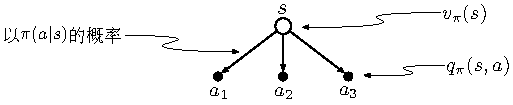
\includegraphics[width=.6\textwidth]{c3/img/state_value_ito_action_value.pdf}
\end{center}
依据这一直观感受与给出的逆流图, 请写出这样的等式: 其使用叶结点的值$q_{\pi}(s, a)$(给定$S_t = s$)来表示根结点的值$v_{\pi}(s)$. 这一等式应该包括基于策略$\pi$的期望式. 然后给出第二个等式, 其中期望式使用$\pi(a \mid s)$展开, 使得等式中没有期望符号.
\end{exer}

\begin{exer}
一个动作的值, $q_{\pi}(s, a)$, 依赖于期望的下一奖赏与期望的余下奖赏的和. 同样, 我们可以通过``以某一动作(动作-状态对)为根, 发散出各个可能的下一状态''的逆流图来理解这一点:
\begin{center}
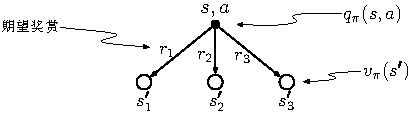
\includegraphics[width=.45\textwidth]{c3/img/action_value_ito_state_value.pdf}
\end{center}
依据这一直观感受与给出的逆流图, 请写出这样的等式: 其使用期望的下一奖赏$R_{t + 1}$与期望的下一状态的值$v_{\pi}(S_{t + 1})$(给定$S_t = s$及$A_t = a$)来表示动作值$q_{\pi}(s, a)$. 这一等式应该包括一个期望式, 但该期望式并\emph{不}基于当下策略. 然后给出第二个等式, 其中期望式使用如\eqref{eq:3.2}定义的$p(s', r \mid s, a)$来展开, 使得该等式中没有期望符号.
\end{exer}

% ----------------------------------- sec3.6 ---------------------------------------------
\section{最优策略与最优值函数}\label{sec:3.6}

粗略地说, 解决强化学习问题即意味着发现能在长期中接高额奖赏的策略. 对于有限MDP来说, 我们可以使用下述的方式精确地定义最优策略. 通过值函数, 我们可以在策略上定义一个偏序关系. 如果在所有的状态上, 使用策略$\pi$获得的期望回报都高于或等于策略$\pi'$, 则策略$\pi$被定义为优于策略$\pi'$. 换句话说, $\pi \geq \pi'$当且仅当$v_{\pi}(s) \geq v_{\pi'}(s)$对所有的$s \in \mathcal{S}$成立. 总有一个策略优于或其他的所有策略或和其他的所有策略一样好. 这就是\emph{最优策略}<optimal policy>. 虽然可能有不止一个的最优策略, 但我们将所有的最优策略都记为$\pi_{*}$. 这些最优策略都有着相同的状态值函数, 该状态值函数称为\emph{最优状态值函数}<optimal state-value function>, 记为$v_*$, 定义如下:
\begin{equation}\label{eq:3.15}
v_*(s) \doteq \max_{\pi}v_{\pi}(s),
\end{equation}
对所有的$s \in \mathcal{S}$成立.

最优策略也共享着相同的\emph{最优动作值函数}<optimal action-value function>, 其记为$q_*$, 且定义如下:
\begin{equation}\label{eq:3.16}
q_*(s, a) \doteq \max_{\pi}q_{\pi}(s, a),
\end{equation}
对所有的$s \in \mathcal{S}$与$a \in \mathcal{A}(s)$成立. 对状态-动作对$(s, a)$来说, 这一函数定义了在状态$s$下采取动作$a$, 并在之后遵循最优策略而可以获得的期望回报. 因此, 我们可以如下用$v_*$定义$q_*$:
\begin{equation}\label{eq:3.17}
q_*(s, a) = \mathbb{E}[R_{t + 1} + \gamma v_*(S_{t + 1}) \mid S_t = s, A_t = a].
\end{equation}

\begin{exam}[高尔夫的最优值函数]
\figref{3.3}的下侧展示了可能的最优动作值函数$q_*(s, \mathtt{driver})$的轮廓线. 这些值为, 如果我们先用木杆打一杆, 并在之后选择木杆或推杆两者中较好的那个, 而得到的各个状态的值. 木杆能让我们击出去的球更远, 但会损失准确度. 当使用木杆时, 只有我们离球洞足够近, 我们才能一杆入洞, 因此$q_*(s, \mathtt{driver})$的$-1$的轮廓线只覆盖了果岭的一小部分. 但如果我们能打两杆的话, 我们就可以从远得多的地方击球入洞, 就像$-2$的轮廓线所示的那样. 在这种情形下, 我们不必一直用木杆来进到较小的$-1$轮廓线内, 而只需要进到果岭内; 在那里我们可以使用推杆. 最优动作值函数给出了如下情形下的值: 先采取特定的\emph{最初}动作, 此处即为使用木杆, 之后则一直选择最佳的动作. $-3$的轮廓线是在更外围的地方, 且包括了球座. 从球座起, 最佳的动作序列为先使用两次木杆然后使用一次推杆, 这样就可以将球打入洞中.
\end{exam}

因为$v_*$为某一策略下的值函数, 其必须满足针对状态值的贝尔曼方程\eqref{eq:3.14}所给出的自洽条件. 但因为最优值函数的缘故, $v_*$的一致性条件可以以不参照任何特定策略的特殊形式写出. 这即为针对$v_*$的贝尔曼方程, 或者可以称之为\emph{贝尔曼最优性方程}<Bellman optimality equation>. 直观地看, 贝尔曼最优性方程所表述的事实为: 在最优策略下, 一个状态的值一定等于在该状态下采取最优动作所获得的期望回报:
\begin{align}
v_*(s) &= \max_{a \in \mathcal{A}(s)}q_{\pi_*}(s, a) \nonumber \\
&= \max_a \mathbb{E}_{\pi_*}[G_t \mid S_t = s, A_t = a] \nonumber \\
&= \max_a \mathbb{E}_{\pi_*}[R_{t + 1} + \gamma G_{t + 1} \mid S_t = s, A_t = a] \tag*{\text{通过$\eqref{eq:3.9}$}} \nonumber \\
&= \max_a \mathbb{E}[R_{t + 1} + \gamma v_*(S_{t + 1}) \mid S_t = s, A_t = a] \label{eq:3.18} \\
&= \max_a \sum_{s', r}p(s', r \mid s, a)[r + \gamma v_*(s')] \label{eq:3.19}
\end{align}
最后两个等式是针对$v_*$的贝尔曼最优性方程的两种形式. 针对$q_*$的贝尔曼最优性方程为
\begin{equation}\label{eq:3.20}
\begin{aligned}[b]
q_*(s. a) &= \mathbb{E} \left[ R_{t + 1} + \gamma \max_{a'}q_*(S_{t + 1}, a') \mid S_t = s, A_t = a \right] \\
&= \sum_{s', r} p(s', r \mid s, a) \left[ r + \gamma \max_{a'}q_*(s', a') \right].
\end{aligned}
\end{equation}

\figref{3.4}中的逆流图从图形上展示了针对$v_*$与$q_*$的贝尔曼最优性方程中所考虑的未来状态与动作的范围. 这些逆流图和之前呈现的针对$v_\pi$与$q_\pi$的逆流图类似, 只是在选择点处添加了添加了弧线来表明进行了最优选择, 而不是计算给定策略下的期望值. 图中左侧的逆流图从图形上表示贝尔曼最优性方程\eqref{eq:3.19}, 而右侧的从图形上表示\eqref{eq:3.20}.

\begin{figure}[htb]
\centering
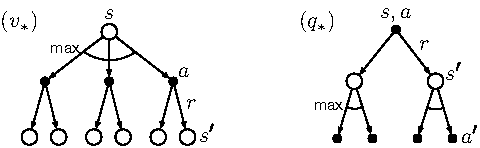
\includegraphics[width=.6\textwidth]{c3/img/figure3-4.pdf}
\caption{针对$v_*$与$q_*$的逆流图}\label{fig:3.4}
\end{figure}

对于有限MDP而言, 针对$v_*$的贝尔曼最优性方程\eqref{eq:3.19}有不依赖于策略的唯一解. 贝尔曼最优性方程实际上是方程组, 每一个状态都对应于一个方程, 因此如果有$n$个状态的话, 那么就在$n$个方程中有$n$个未知数. 如果环境的动态$p$是已知的, 那么原则上说我们可以从各种各样的解非线性方程组的方法中选择一个来求得$v_*$. 同样, 也可以解类似的方程组来求出$q_*$.

一旦我们知道了$v_*$, 那么确定最优策略就相对来说比较容易了. 对每个状态$s$来说, 都有一个或多个动作可以在贝尔曼最优性方程中取得最大值. 任何只将非零的概率分配给这些动作的策略都是最优策略. 你可以将此理解为单步搜索. 如果你已经知道了最优值函数$v_*$, 那么在单步搜索后表现得最好的动作即为最优动作. 另一个看待这一点的视角为: 任一就最优值函数$v_*$而言贪心的策略都是最优策略. 在计算机科学的领域中, 术语贪心用于``只基于局部或当前的考量来进行选择, 而不考虑这样的选择是否会在将来阻碍我们做出更好的选择''这样的搜索或决策过程. 因此, 其用于形容仅基于短期结果来进行动作选择的策略. $v_*$的优美之处在于, 如果我们将其用于对动作的短期结果进行评估——或更确切地说, 单步结果——那么从我们所关注的长期的角度看, 贪婪策略事实上是最优的, 因为$v_*$已经将所有可能的未来动作所产生的关于奖赏的影响考虑在内. 通过$v_*$, 最优的长期期望回报转为了可以在每个状态上通过局部、立即的计算而获得的量. 因此, 单步搜索即可得到长期而言最优的动作.

如果我们知道了$q_*$, 那么选择最优动作甚至可以更简单. 有了$q_*$, 代理甚至都不必进行单步搜索: 对任一状态$s$, 代理可以轻松地发现最大化$q_*(s, a)$的动作. 动作值函数实际上已经存储了所有单步搜索的结果. 其将最优的长期期望回报作为``可以在每一个状态-动作对上立即获得的本地的量''提供. 因此, 以构建动作-状态对上而非状态上的函数为代价, 最优动作值函数使得我们可以选择最优动作而不必了解任何和可能的后一状态与后一状态的值有关的信息, 即不必了解关于环境的动态的任何信息.

\begin{exam}[解决网格世界问题]
对于在\examref{3.5}中介绍的简单的网格问题, 我们将其在\figref{3.5}(左)中再次进行展示, 并假设我们已经解得了针对$v_*$的贝尔曼方程. 让我们回想一下, 紧随状态\textsf{A}的是+10的奖赏以及到状态\textsf{A'}的转移, 而紧随状态\textsf{B}的是+5的奖赏以及到状态\textsf{B'}的转移. \figref{3.5}(中)展示了最优值函数, 而\figref{3.5}(右)展示了对应的最优策略. 有些小方格内有多个箭头, 则所有这些箭头对应的动作都是最优的.
\begin{figure}[H]
\centering
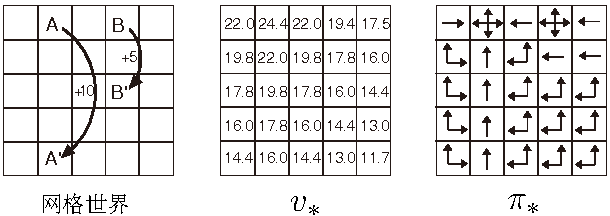
\includegraphics[width=.8\textwidth]{c3/img/figure3-5.pdf}
\caption{网格世界例子的最优解}\label{fig:3.5}
\end{figure}
\vspace{-2em}
\end{exam}

\begin{exam}[回收机器人问题上的贝尔曼最优性方程]
使用\eqref{eq:3.19}, 我们可以明确地给出回收机器人例子上的贝尔曼最优性方程. 简洁起见, 我们将状态\texttt{high}, \texttt{low}以及动作\texttt{search}, \texttt{wait}, \texttt{recharge}分别记为\texttt{h}, \texttt{l}, \texttt{s}, \texttt{w}, \texttt{re}. 因为只有两个状态, 因此贝尔曼最优性方程包含了两个方程. 针对$v_*(\mathtt{h})$的方程可以写作:
\begin{equation*}
\newcommand{\tth}{\mathtt{h}}
\newcommand{\tts}{\mathtt{s}}
\newcommand{\ttl}{\mathtt{l}}
\newcommand{\ttw}{\mathtt{w}}
\begin{aligned}[b]
v_*(h) &= \max \left.
\begin{cases}
&p(\tth \mid \tth, \tts) [r(\tth, \tts, \tth) + \gamma v_*(\tth)] + p(\ttl \mid \tth, \tts)[r(\tth, \tts, \ttl) + \gamma v_*(\ttl)], \\
&p(\tth \mid \tth, \ttw) [r(\tth, \ttw, \tth) + \gamma v_*(\tth)] + p(\ttl \mid \tth, \ttw)[r(\tth, \ttw, \ttl) + \gamma v_*(\ttl)]
\end{cases} \right\} \\
&= \max \left.
\begin{cases}
&\alpha [r_\tts + \gamma v_*(\tth)] + (1 - \alpha)[r_\tts + \gamma v_*(\ttl)], \\
&1[r_\ttw + \gamma v_*(\tth)] + 0[r_\ttw + \gamma v_*(\ttl)]
\end{cases} \right\} \\
&=\max \left.
\begin{cases}
&r_\tts + \gamma[\alpha v_*(\tth) + (1 - \alpha)v_*(\ttl)], \\
&r_\ttw + \gamma v_*(\tth)
\end{cases} \right\}.
\end{aligned}
\end{equation*}
如果$v_*(\mathtt{l})$也沿用同样的流程的话, 将得到如下的方程
\begin{equation*}
\newcommand{\tth}{\mathtt{h}}
\newcommand{\tts}{\mathtt{s}}
\newcommand{\ttl}{\mathtt{l}}
\newcommand{\ttw}{\mathtt{w}}
v_*(\ttl) = \max \left.
\begin{cases}
&\beta r_\tts - 3(1 - \beta) + \gamma [(1 - \beta)v_*(\tth) + \beta v_*(\ttl)], \\
&r_\ttw + \gamma v_*(\ttl), \\
&\gamma v_*(\tth)
\end{cases} \right\}.
\end{equation*}
对于任何满足$0 \leq \gamma < 1$, $0 \leq \alpha, \beta \leq 1$这两个条件的$r_\mathtt{s}$, $r_\mathtt{w}$, $\alpha$, $\beta$以及$\gamma$的取值, 总是恰好有一对解$v_*(\mathtt{h})$与$v_*(\mathtt{l})$, 同时满足上述的两个非线性方程.
\end{exam}

显式地求解贝尔曼最优性方程为我们提供了一个获得最优策略的方法, 亦即提供了一个解决强化学习问题的方法. 然而, 这一解决方案很少能直接派上用场. 其类似于穷举搜索, 其需要考虑所有的可能性, 计算各个可能性发生的概率以及就期望奖赏而言的吸引力. 这一解决方案依赖于至少3个很少在应用中成立的假设: (1) 我们准确地知道环境的动态; (2) 我们有足够的算力来完成对这一方案的求解; 以及(3) 马尔科夫性质. 对于我们所感兴趣的各种各样的任务, 我们通常不能使用这一解法, 因为这些假设的某一个组合可能无法得到满足. 例如, 对西洋双陆棋而言, 虽然第一条与第三条假设不成问题, 但第二条假设是重大的阻碍. 因为该游戏有大约$10^{20}$个状态, 如今最快的计算机也需要花费数千年来解得针对$v_*$的贝尔曼方程, 对求解$q_*$而言同样如此. 在强化学习中, 通常我们需要将就于近似解. 

许多不同的决策方法, 可以被视为近似地解贝尔曼最优性方程的手段. 例如, 启发式搜索可以被视为将\eqref{eq:3.19}的右侧展开数次直至一定的深度, 形成一棵可能性的``树'', 然后使用启发式的评估函数来近似位于``叶''结点的$v_*$. (例如$\mathrm{A}^*$的启发式搜索方法几乎总是基于分节式情形.) 动态规划方法和贝尔曼最优性方程的关联甚至更为紧密. 许多强化学习方法可以明确地被理解为, 使用实际经历到的转移来代替关于期望转移的知识, 以近似地求解贝尔曼最优性方程. 我们将在接下来的几章中考虑各种这样的方法.

\begin{exer}
对于高尔夫的例子, 画出或描述出其最优状态值函数.
\end{exer}

\begin{exer}
对于高尔夫的例子, 画出或描述出关于推球的最优动作值函数$q_*(s, \mathtt{putter})$.
\end{exer}

\vspace{-2em}
\begin{wrapfigure}{r}{.3\textwidth}
\centering
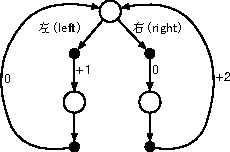
\includegraphics[width=.3\textwidth]{c3/img/exercise3-22.pdf}
\end{wrapfigure}
\mbox{}~
\begin{exer}
考虑如右图所示的持续式MDP. 顶部的状态中有唯一需要作出的决定, 其中可以采取两个动作, \textsf{left}以及\textsf{right}. 图中数字为采取动作后接收到的确定性奖赏. 仅有两个确定性的策略, $\pi_{\mathsf{left}}$与$\pi_{\mathsf{right}}$. 如果$\gamma = 0$的话哪个策略是最优的? 如果$\gamma = 0.9$呢? 或如果$\gamma = 0.5$呢?
\end{exer}

\begin{exer}
关于回收机器人, 给出针对$q_*$的贝尔曼方程.
\end{exer}

\begin{exer}
\figref{3.5}显示出, 在网格世界中, 最佳的状态的最优值为24.4(保留1位有效数字). 使用关于最优策略与\eqref{eq:3.8}的知识, 来用数学表达式表示这个值, 并将该值计算到3位有效数字. 
\end{exer}

\begin{exer}
给出一个使用$q_*$来表示$v_*$的等式.
\end{exer}

\begin{exer}
给出一个使用$v_*$与4参数函数$p$来表示$q_*$的等式.
\end{exer}

\begin{exer}
给出一个使用$q_*$来表示$\pi_*$的等式.
\end{exer}

\begin{exer}
给出一个使用$v_*$与4参数函数$p$来表示$\pi_*$的等式.
\end{exer}

\begin{exer}
使用3参数函数$p$\eqref{eq:3.4}以及2参数函数$r$, 来重写针对4种值函数($v_\pi$, $v_*$, $q_\pi$, $q_*$)的贝尔曼方程.
\end{exer}

% ----------------------------------- sec3.7 ---------------------------------------------
\section{最优性与近似}\label{sec:3.7}

我们已经定义了最优值函数与最优策略. 很明显, 学得了最优策略的代理将表现得非常好, 但在实际中这很少发生. 在我们所关心的各种问题中, 只有通过极端的计算开销才能获得最优策略. 对最优性的规范的见解, 可以帮助梳理本书中介绍的强化学习方法, 并为帮助我们理解各种学习算法的理论性质提供了一种途径, 但最优性仅是代理可以在不同程度上接近的一种理想化. 正如我们前面所讨论的, 即使我们拥有对环境的完整而准确的模型, 通过单纯地解贝尔曼最优性方程来得到最优策略通常是不现实的. 举个例子, 棋类游戏, 如国际象棋, 仅占到人类各种经验的极小的一部分, 但是规模庞大的定制计算机也无法计算出最优下法. 代理所面临的问题中极为关键的一个方面为其拥有多少算力, 更具体地说, 其能在一个时步中完成多少计算.

内存的大小也是一个重要的制约. 通常, 为了建立起对值函数、策略以及模型的估计, 通常需要大量的内存. 如果任务的状态集小而有限, 那么使用数组或表格<table>来进行估计是可行的, 其中各个状态(或状态-动作对)都有对应的表项. 我们将此称为\emph{表格式}情形, 并将对应的方法称为表格式方法. 而在我们感兴趣的许多实际情形下, 状态的数量太多了而远不能放入表格内. 在这种情形下, 我们必须使用某种简洁的参数化函数表示方法, 来对函数进行近似.

我们关于强化学习问题的框架迫使我们将就于使用近似. 然而, 其也为我们提供了独特机会用以达成合格近似. 例如, 在对近似求解最优动作时, 可能有很多状态代理遇到的概率非常小, 以至在这些状态上选择次优动作对代理接收到的奖赏总量几乎没有影响. 例如, Tesauro的西洋双陆棋程序拥有卓越的技巧, 哪怕其在面临不会在和高手的对战中出现的场景时, 有可能做出极糟糕的决策. 事实上, 极有可能TD-Gammon在游戏状态集的一大部分中都做出糟糕的决策. 强化学习的在线特性使得可以以这样的方式来近似最优策略: 在经常遇到的状态上投入更多的精力, 使得能在这些状态上做出好的决策——以在不常遇到的状态上投入更少精力为代价. 这是将强化学习同其他的近似求解MDP的方法区分开来的一个关键特性.

% ----------------------------------- sec3.8 ---------------------------------------------
\section{总结}\label{sec:3.8}

让我们总结下呈现在本章中的强化学习问题诸要素. 强化学习的目标从交互中学习如何决策以达成目的. 强化学习的\emph{代理}与其\emph{环境}在一系列离散的时步上交互. 两者接口间的具体细节定义出了具体的任务: \emph{动作}是需要由代理作出的选择; \emph{状态}为决策的基础; \emph{奖赏}是对做出的决策进行评估的基础. 代理内部的一切都为代理彻底知晓与控制; 而代理外部的一切可以被代理部分控制, 但为代理彻底知晓与否是不确定的. \emph{策略}为一概率性规则, 通过这个规则代理将动作作为状态的函数来进行选择. 代理的目标即为最大化随时间流逝所接收到的累积奖赏.

如果上述的强化学习设定与明确定义的转移概率一同表述, 那么就构成了\emph{马尔科夫决策过程}(MDP). 有限MDP为拥有有限状态集、有限动作集以及(于此处提出的)有限奖赏集的MDP. 当前强化学习的多数理论都限定于有限MDP, 但是这些方法与理念可以应用于更一般的情形.

\emph{回报}是未来的奖赏的函数, 也是代理寻求最大化的目标(从期望的角度). 取决于任务的特性以及我们是否希望对延迟的奖赏进行折扣, 其有数种不同的定义. 非折扣形式适合于\emph{分节式任务}, 在分节式任务中代理与环境间的交互可以自然地划分成不同的分节; 折扣形式适合于\emph{持续式任务}, 在持续式任务中交互不能自然地划分为不同的分节, 而是无限地持续下去. 我们希望统一两类任务中回报的定义, 使得同一套公式可以同时适用于分节式情形与连续式情形.

一策略的\emph{值函数}为每个状态(或状态-动作对)给出了在该策略下, 从该状态(或状态-动作对)起可以获得的期望回报. \emph{最优值函数}为每个状态(或状态-动作对)给出了各个策略中所能获得的最大期望回报. 值函数为最优的策略即为\emph{最优策略}. 对一个给定的MDP, 虽然针对状态或状态-动作对的最优值函数是唯一的, 但可能有多个最优策略. 任何就最优值函数而言贪心的策略一定是最优策略. \emph{贝尔曼最优性方程}为最优值函数必须满足的特殊一致性条件, 并且从理论上说, 我们可以从中解得最优值函数, 然后利用最优值函数我们可以相对轻松地确定最优策略.

取决于对代理起始时所拥有的关于环境的知识水平的不同假设, 强化学习问题可以以多种不同的方式呈现. 在有\emph{完全知识}的问题中, 代理有完整而准确的环境模型. 如果该环境为MDP, 那么模型应该包括4参数动态函数$p$\eqref{eq:3.2}. 而在\emph{不完全知识}的问题中, 无法获得完整且完美的环境模型.

即使代理有完整而准确的环境模型, 代理通常无法进行足够多的计算来彻底对其进行利用. 可以获得的内存的大小也是一个重要的制约因素. 我们可以需要内存来建立起对值函数、策略以及模型的准确估计. 在实际感兴趣的多数情形下, 状态通常太多了而无法放入表中, 此时必须进行函数近似.

对最优性的规范的见解, 可以帮助梳理本书中介绍的强化学习方法, 并为帮助我们理解各种学习算法的理论性质提供了一种途径, 但最优性仅是代理可以在不同程度上接近的一种理想化. 在强化学习中我们十分关心最优解不能被被找到, 但可以以某种方法被近似的情形. 

% ----------------------------------- bib ---------------------------------------------
\section*{参考文献与历史沿革}

暂不译